\documentclass[ignorenonframetext,]{beamer}
\setbeamertemplate{caption}[numbered]
\setbeamertemplate{caption label separator}{: }
\setbeamercolor{caption name}{fg=normal text.fg}
\beamertemplatenavigationsymbolsempty
\usepackage{lmodern}
\usepackage{amssymb,amsmath}
\usepackage{ifxetex,ifluatex}
\usepackage{fixltx2e} % provides \textsubscript
\ifnum 0\ifxetex 1\fi\ifluatex 1\fi=0 % if pdftex
  \usepackage[T1]{fontenc}
  \usepackage[utf8]{inputenc}
\else % if luatex or xelatex
  \ifxetex
    \usepackage{mathspec}
  \else
    \usepackage{fontspec}
  \fi
  \defaultfontfeatures{Ligatures=TeX,Scale=MatchLowercase}
\fi
% use upquote if available, for straight quotes in verbatim environments
\IfFileExists{upquote.sty}{\usepackage{upquote}}{}
% use microtype if available
\IfFileExists{microtype.sty}{%
\usepackage{microtype}
\UseMicrotypeSet[protrusion]{basicmath} % disable protrusion for tt fonts
}{}
\newif\ifbibliography
\hypersetup{
            pdftitle={Random Effects ANCOVA},
            pdfborder={0 0 0},
            breaklinks=true}
\urlstyle{same}  % don't use monospace font for urls
\usepackage{color}
\usepackage{fancyvrb}
\newcommand{\VerbBar}{|}
\newcommand{\VERB}{\Verb[commandchars=\\\{\}]}
\DefineVerbatimEnvironment{Highlighting}{Verbatim}{commandchars=\\\{\}}
% Add ',fontsize=\small' for more characters per line
\usepackage{framed}
\definecolor{shadecolor}{RGB}{248,248,248}
\newenvironment{Shaded}{\begin{snugshade}}{\end{snugshade}}
\newcommand{\KeywordTok}[1]{\textcolor[rgb]{0.13,0.29,0.53}{\textbf{#1}}}
\newcommand{\DataTypeTok}[1]{\textcolor[rgb]{0.13,0.29,0.53}{#1}}
\newcommand{\DecValTok}[1]{\textcolor[rgb]{0.00,0.00,0.81}{#1}}
\newcommand{\BaseNTok}[1]{\textcolor[rgb]{0.00,0.00,0.81}{#1}}
\newcommand{\FloatTok}[1]{\textcolor[rgb]{0.00,0.00,0.81}{#1}}
\newcommand{\ConstantTok}[1]{\textcolor[rgb]{0.00,0.00,0.00}{#1}}
\newcommand{\CharTok}[1]{\textcolor[rgb]{0.31,0.60,0.02}{#1}}
\newcommand{\SpecialCharTok}[1]{\textcolor[rgb]{0.00,0.00,0.00}{#1}}
\newcommand{\StringTok}[1]{\textcolor[rgb]{0.31,0.60,0.02}{#1}}
\newcommand{\VerbatimStringTok}[1]{\textcolor[rgb]{0.31,0.60,0.02}{#1}}
\newcommand{\SpecialStringTok}[1]{\textcolor[rgb]{0.31,0.60,0.02}{#1}}
\newcommand{\ImportTok}[1]{#1}
\newcommand{\CommentTok}[1]{\textcolor[rgb]{0.56,0.35,0.01}{\textit{#1}}}
\newcommand{\DocumentationTok}[1]{\textcolor[rgb]{0.56,0.35,0.01}{\textbf{\textit{#1}}}}
\newcommand{\AnnotationTok}[1]{\textcolor[rgb]{0.56,0.35,0.01}{\textbf{\textit{#1}}}}
\newcommand{\CommentVarTok}[1]{\textcolor[rgb]{0.56,0.35,0.01}{\textbf{\textit{#1}}}}
\newcommand{\OtherTok}[1]{\textcolor[rgb]{0.56,0.35,0.01}{#1}}
\newcommand{\FunctionTok}[1]{\textcolor[rgb]{0.00,0.00,0.00}{#1}}
\newcommand{\VariableTok}[1]{\textcolor[rgb]{0.00,0.00,0.00}{#1}}
\newcommand{\ControlFlowTok}[1]{\textcolor[rgb]{0.13,0.29,0.53}{\textbf{#1}}}
\newcommand{\OperatorTok}[1]{\textcolor[rgb]{0.81,0.36,0.00}{\textbf{#1}}}
\newcommand{\BuiltInTok}[1]{#1}
\newcommand{\ExtensionTok}[1]{#1}
\newcommand{\PreprocessorTok}[1]{\textcolor[rgb]{0.56,0.35,0.01}{\textit{#1}}}
\newcommand{\AttributeTok}[1]{\textcolor[rgb]{0.77,0.63,0.00}{#1}}
\newcommand{\RegionMarkerTok}[1]{#1}
\newcommand{\InformationTok}[1]{\textcolor[rgb]{0.56,0.35,0.01}{\textbf{\textit{#1}}}}
\newcommand{\WarningTok}[1]{\textcolor[rgb]{0.56,0.35,0.01}{\textbf{\textit{#1}}}}
\newcommand{\AlertTok}[1]{\textcolor[rgb]{0.94,0.16,0.16}{#1}}
\newcommand{\ErrorTok}[1]{\textcolor[rgb]{0.64,0.00,0.00}{\textbf{#1}}}
\newcommand{\NormalTok}[1]{#1}
\usepackage{graphicx,grffile}
\makeatletter
\def\maxwidth{\ifdim\Gin@nat@width>\linewidth\linewidth\else\Gin@nat@width\fi}
\def\maxheight{\ifdim\Gin@nat@height>\textheight0.8\textheight\else\Gin@nat@height\fi}
\makeatother
% Scale images if necessary, so that they will not overflow the page
% margins by default, and it is still possible to overwrite the defaults
% using explicit options in \includegraphics[width, height, ...]{}
\setkeys{Gin}{width=\maxwidth,height=\maxheight,keepaspectratio}

% Prevent slide breaks in the middle of a paragraph:
\widowpenalties 1 10000
\raggedbottom

\AtBeginPart{
  \let\insertpartnumber\relax
  \let\partname\relax
  \frame{\partpage}
}
\AtBeginSection{
  \ifbibliography
  \else
    \let\insertsectionnumber\relax
    \let\sectionname\relax
    \frame{\sectionpage}
  \fi
}
\AtBeginSubsection{
  \let\insertsubsectionnumber\relax
  \let\subsectionname\relax
  \frame{\subsectionpage}
}

\setlength{\parindent}{0pt}
\setlength{\parskip}{6pt plus 2pt minus 1pt}
\setlength{\emergencystretch}{3em}  % prevent overfull lines
\providecommand{\tightlist}{%
  \setlength{\itemsep}{0pt}\setlength{\parskip}{0pt}}
\setcounter{secnumdepth}{0}

\title{Random Effects ANCOVA}
\date{}

\begin{document}
\frame{\titlepage}

\begin{frame}{ANCOVA}

\begin{quote}
``What's in a name? That which we call a rose\\
By any other name would smell as sweet.''

\hfill --- Romeo and Juliet II, ii, 1-2
\end{quote}

\begin{figure}
\centering
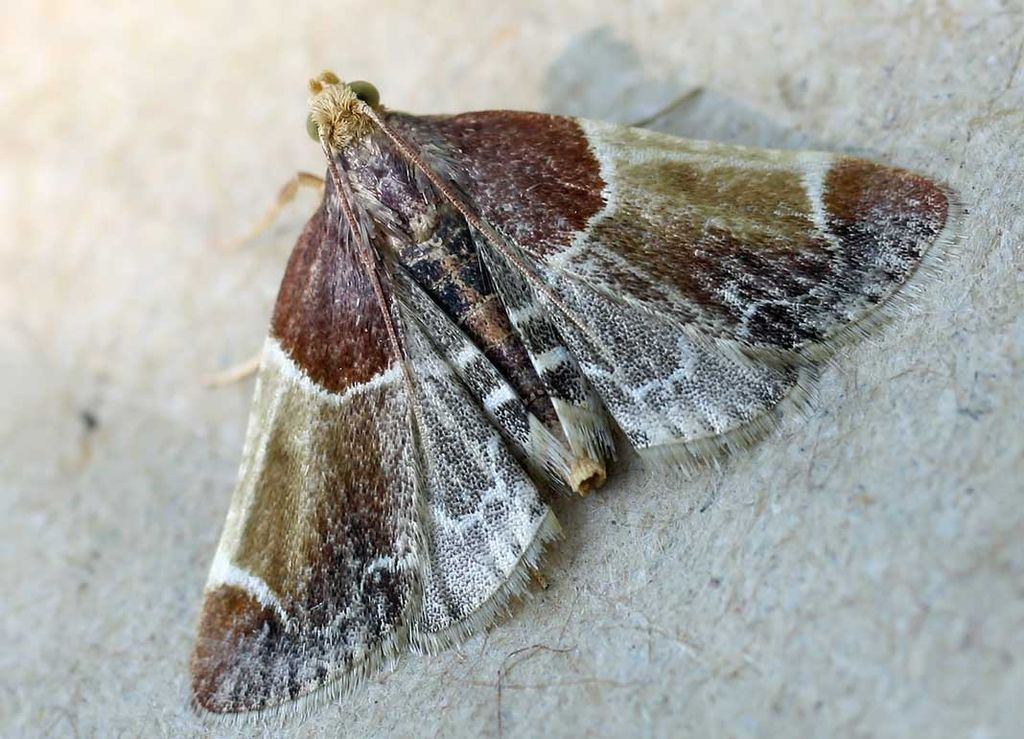
\includegraphics[width=0.40000\textwidth]{figures/ancovamoth.jpg}
\caption{Ancova moth, or snout moth}
\end{figure}

ANOVA, ANCOVA, MANOVA -- what's the difference?

\end{frame}

\begin{frame}{}

\begin{itemize}
\item
  ANOVA (Analysis of Variance): continuous outcome, categorical
  predictor(s)

  \begin{itemize}
  \tightlist
  \item
    one-way ANOVA: one categorical predictor
  \item
    two-way ANOVA: two categorical predictors
  \item
    two-way ANOVA with interaction: you get the picture!
  \end{itemize}
\item
  ANCOVA (Analysis of Covariance): continuous outcome, categorical
  predictor(s), at least one continuous predictor that is generally
  considered a nuisance (not unlike the snout moths, which are often
  considered pests because they share our tastes in grains)
\item
  MANOVA (Multivariate ANOVA): multiple continuous outcomes, categorical
  predictor(s)
\end{itemize}

Historically these names had implications regarding the estimation
methods used, but that is no longer always the case.

\end{frame}

\begin{frame}{Motivating Example: National Educational Longitudinal
Study of Education (NELS)}

Hoff considers a subset of the NELS data that contains information on
math scores of a random sample of 10th graders selected from a national
sample of 100 large urban public schools. We plot the math scores
\(y_{ij}\) of the \(n_j\) students in each school \(j\), ranked by the
average score.

\end{frame}

\begin{frame}{}

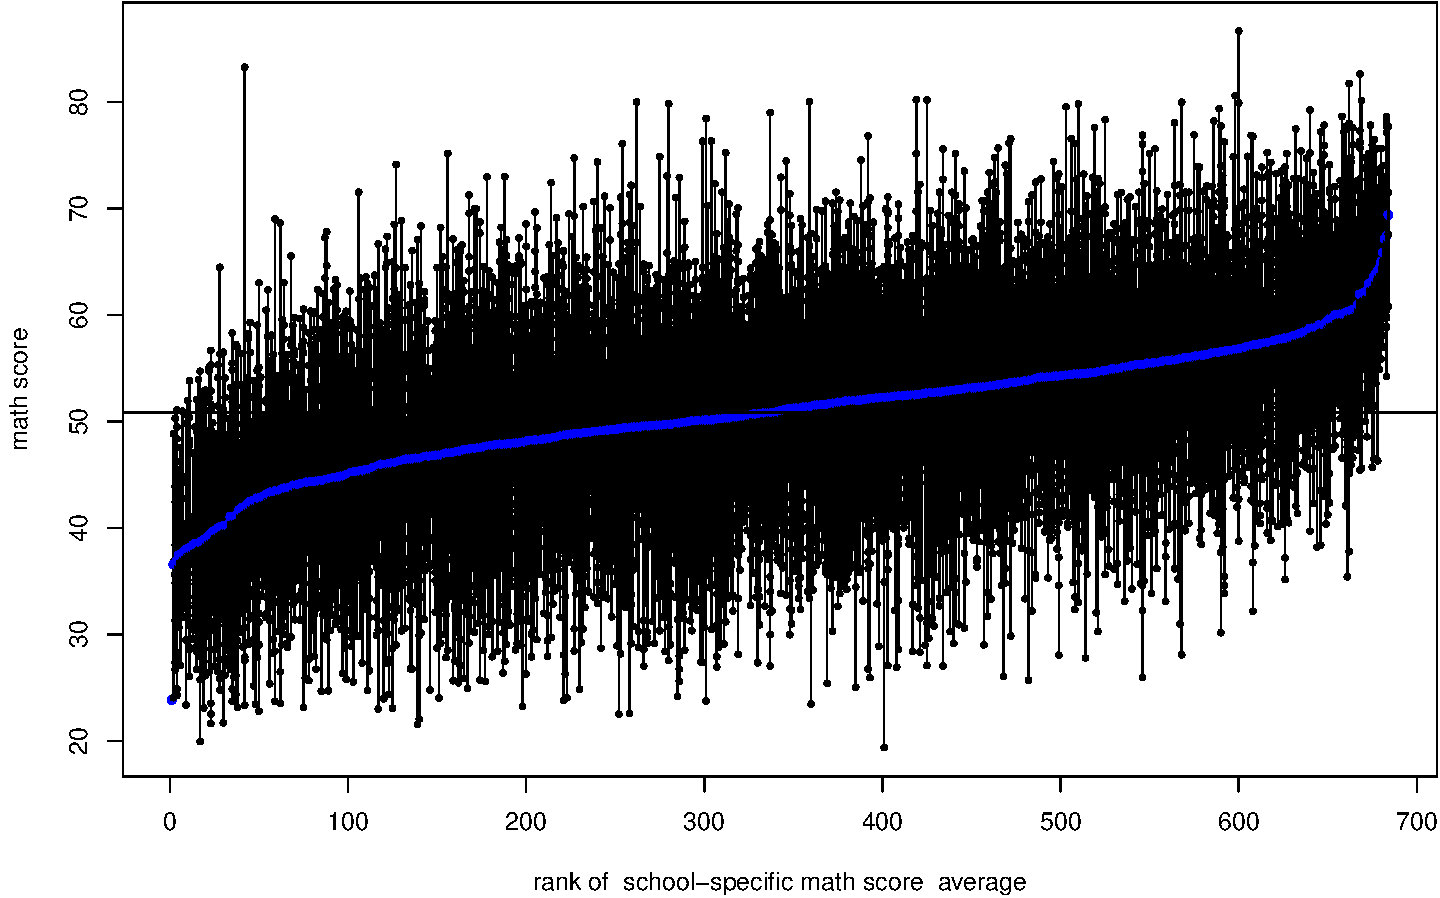
\includegraphics{anova_06_deck_files/figure-beamer/nelsplot1-1.pdf}

\end{frame}

\begin{frame}{}

\begin{itemize}
\item
  The school-specific averages range from 36.58 to 65.02, with 48.13 the
  average of all 100 school averages (weighting each school equally).
\item
  The school-specific variances range from 21.81 to 179.69 -- quite a
  wide range!
\item
  The school with the highest average only contains 4 observations.
\end{itemize}

\end{frame}

\begin{frame}{Which school is best?}

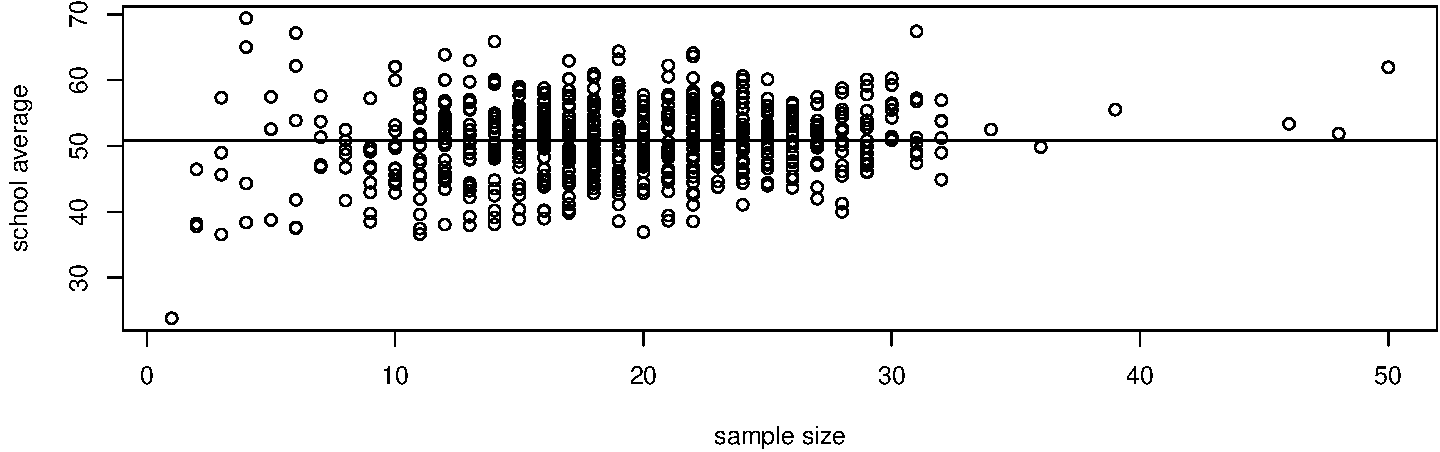
\includegraphics{anova_06_deck_files/figure-beamer/nelsplot2-1.pdf}

Note that the school with the highest average has the smallest sample
size (\(n_j=4\)). Do we have strong evidence that the true mean in this
school is substantially larger than that in other schools in the sample?
How might we answer this question?

\end{frame}

\begin{frame}[fragile]{ANOVA}

One approach would be to fit a fixed effects ANOVA model:

\begin{Shaded}
\begin{Highlighting}[]
\NormalTok{m1=}\KeywordTok{lm}\NormalTok{(nels_mathdat}\OperatorTok{$}\NormalTok{mscore}\OperatorTok{~}\KeywordTok{as.factor}\NormalTok{(nels_mathdat}\OperatorTok{$}\NormalTok{school)}\OperatorTok{-}\DecValTok{1}\NormalTok{)}
\KeywordTok{anova}\NormalTok{(m1)}
\end{Highlighting}
\end{Shaded}

\begin{verbatim}
## Analysis of Variance Table
## 
## Response: nels_mathdat$mscore
##                                   Df   Sum Sq Mean Sq F value    Pr(>F)
## as.factor(nels_mathdat$school)   684 34306852   50156  681.54 < 2.2e-16
## Residuals                      12290   904450      74                  
##                                   
## as.factor(nels_mathdat$school) ***
## Residuals                         
## ---
## Signif. codes:  0 '***' 0.001 '**' 0.01 '*' 0.05 '.' 0.1 ' ' 1
\end{verbatim}

Here we see clear evidence of heterogeneity in math scores across
schools.

\end{frame}

\begin{frame}[fragile]{ANOVA results}

\begin{Shaded}
\begin{Highlighting}[]
\KeywordTok{library}\NormalTok{(sjPlot)}
\KeywordTok{plot_model}\NormalTok{(m1,}\DataTypeTok{sort.est=}\OtherTok{TRUE}\NormalTok{)}
\end{Highlighting}
\end{Shaded}

\end{frame}

\begin{frame}{}

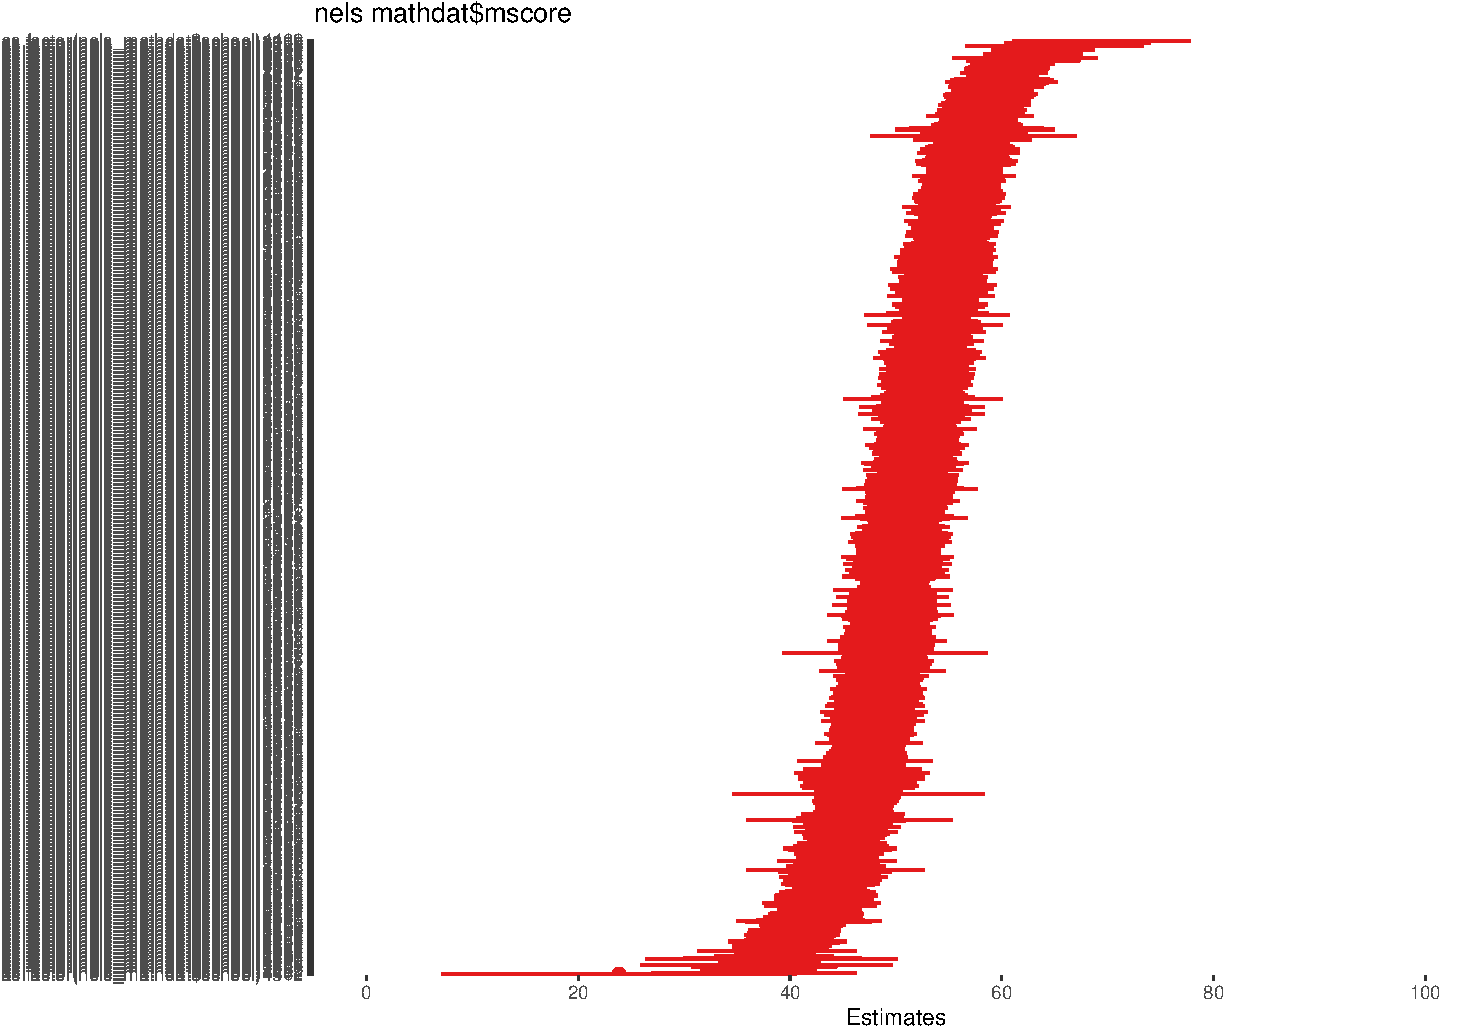
\includegraphics{anova_06_deck_files/figure-beamer/catplot1-1.pdf}

Based on these estimates, we might conclude that the school has higher
performance than some, but not all, schools.

\end{frame}

\begin{frame}[fragile]{Random effects ANOVA}

Note in the prior plot that the highest estimated mean also has a very
large variance. We may wish to use shrinkage estimation in order to
stabilize that and other estimates for schools in which few students
provide data. A random effects ANOVA model is given by
\[y_{ij}=\mu+\alpha_j+\varepsilon_{ij},\] where
\(\varepsilon_{ij} \sim N(0,\sigma^2)\) and
\(\alpha_j \sim N(0,\tau^2)\).

\begin{Shaded}
\begin{Highlighting}[]
\KeywordTok{library}\NormalTok{(lme4)}
\NormalTok{m2=}\KeywordTok{lmer}\NormalTok{(mscore}\OperatorTok{~}\NormalTok{(}\DecValTok{1}\OperatorTok{|}\NormalTok{school),}\DataTypeTok{data=}\NormalTok{nels_mathdat)}
\KeywordTok{summary}\NormalTok{(m2)}
\KeywordTok{library}\NormalTok{(sjstats)}
\KeywordTok{icc}\NormalTok{(m2)}
\end{Highlighting}
\end{Shaded}

\end{frame}

\begin{frame}[fragile]{}

\begin{verbatim}
## Linear mixed model fit by REML ['lmerMod']
## Formula: mscore ~ (1 | school)
##    Data: nels_mathdat
## 
## REML criterion at convergence: 93914.6
## 
## Scaled residuals: 
##     Min      1Q  Median      3Q     Max 
## -3.8113 -0.6534  0.0094  0.6732  4.7000 
## 
## Random effects:
##  Groups   Name        Variance Std.Dev.
##  school   (Intercept) 23.68    4.866   
##  Residual             73.71    8.585   
## Number of obs: 12974, groups:  school, 684
## 
## Fixed effects:
##             Estimate Std. Error t value
## (Intercept)  50.9390     0.2028   251.2
\end{verbatim}

\begin{verbatim}
## # Intraclass Correlation Coefficient
## 
##      Adjusted ICC: 0.243
##   Conditional ICC: 0.243
\end{verbatim}

\end{frame}

\begin{frame}[fragile]{}

Here we examine the distribution of random effects.

\begin{Shaded}
\begin{Highlighting}[]
\KeywordTok{library}\NormalTok{(merTools)}
\KeywordTok{plotREsim}\NormalTok{(}\KeywordTok{REsim}\NormalTok{(m2,}\DataTypeTok{n.sims=}\DecValTok{100}\NormalTok{),}\DataTypeTok{stat=}\StringTok{'median'}\NormalTok{,}\DataTypeTok{sd=}\OtherTok{TRUE}\NormalTok{)}
\end{Highlighting}
\end{Shaded}

\end{frame}

\begin{frame}{}

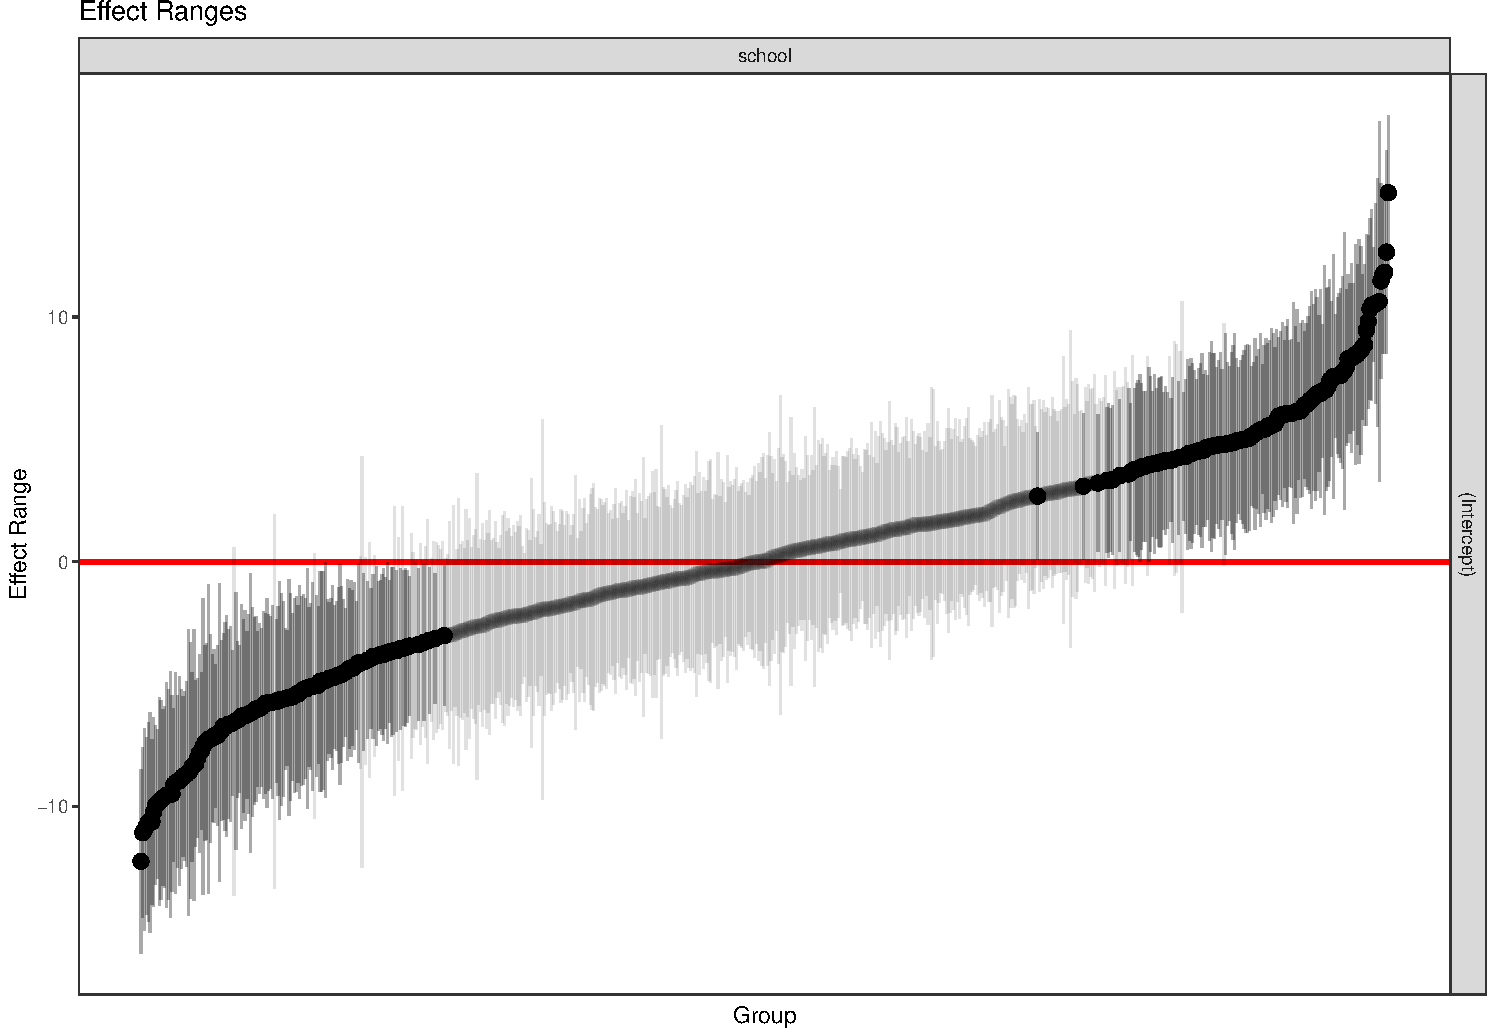
\includegraphics{anova_06_deck_files/figure-beamer/plotre2-1.pdf}

\end{frame}

\begin{frame}{}

How do we conduct a formal test of heterogeneity in this random effects
setting? Well, this is a bit more complicated than in the fixed effects
setting. In particular, no heterogeneity corresponds to the case in
which \(\tau^2=0 \iff \alpha_1=\ldots=\alpha_J=0\), so saying something
about the single parameter \(\tau^2\) has implications about the J
parameters \(\alpha_j\).

A second problem is that \(\tau^2\) cannot be \(<0\), and we wish to
test \(H_0: \tau^2=0\), so we're conducting a hypothesis test at the
boundary of the parameter space instead of in the interior (which would
be the case for \(H_0: \mu=0\)).

\end{frame}

\begin{frame}{}

As shown in Stram and Lee (1994), the approximate asymptotic null
distribution for \(H_0: \tau^2=0\) using a likelihood ratio test
comparing our model to a model with out random effects
(\(y_{ij}=\mu+\varepsilon_{ij}\)) in this case is a 50-50 mixture of a
\(\chi^2_0\) (point mass on 0) and a \(\chi_1^2\) distribution.

\end{frame}

\begin{frame}{}

In general, if we wish to compare a model with \(q+1\) random effects
(calculated as terms that have a random effect, not the number of
groups) to a nested model with \(q\) random effects, the asymptotic null
distribution is a 50-50 mixture of \(\chi^2_{q+1}\) and \(\chi^2_q\)
distributions.

\end{frame}

\begin{frame}{}

Letting LR denote twice the difference in maximized log-likelihoods in
the model with and without a single random effect, you can obtain the
null density in R using
\[0.5*(\text{dchisq}(x,q+1)+\text{dchisq}(x,q))\] and the p-value via
\[0.5*(1-\text{pchisq(LR,q+1)}+1-\text{pchisq}(LR,q)).\]

\end{frame}

\begin{frame}[fragile]{}

For the NELS data fit using a frequentist random effects model, we would
calculate this as follows.

\begin{Shaded}
\begin{Highlighting}[]
\NormalTok{m3=}\KeywordTok{lmer}\NormalTok{(mscore}\OperatorTok{~}\NormalTok{(}\DecValTok{1}\OperatorTok{|}\NormalTok{school),}\DataTypeTok{data=}\NormalTok{nels_mathdat,}\DataTypeTok{REML=}\OtherTok{FALSE}\NormalTok{)}
\NormalTok{m4=}\KeywordTok{lm}\NormalTok{(mscore}\OperatorTok{~}\DecValTok{1}\NormalTok{,}\DataTypeTok{data=}\NormalTok{nels_mathdat)}
\NormalTok{LR=}\KeywordTok{logLik}\NormalTok{(m3)}\OperatorTok{-}\KeywordTok{logLik}\NormalTok{(m4)}
\FloatTok{0.5}\OperatorTok{*}\NormalTok{(}\DecValTok{1}\OperatorTok{-}\KeywordTok{pchisq}\NormalTok{(LR[}\DecValTok{1}\NormalTok{],}\DecValTok{1}\NormalTok{)}\OperatorTok{+}\DecValTok{1}\OperatorTok{-}\KeywordTok{pchisq}\NormalTok{(LR[}\DecValTok{1}\NormalTok{],}\DecValTok{0}\NormalTok{))}
\end{Highlighting}
\end{Shaded}

\begin{verbatim}
## [1] 0
\end{verbatim}

We conclude that there is significant heterogeneity across schools in
the mean math scores.

\end{frame}

\begin{frame}{Bringing SES into the mix}

NELS contains a measure of socioeconomic status (SES) for each student.
We generally expect some degree of correlation between SES and math
score (people who are good at math often can get good jobs, and then
have kids who may inherit math talents; rich parents may have more time
and resources to devote to their kids), though of course the
relationship is not deterministic (there are plenty of math whizzes who
did not have rich parents -- Gauss!, and there are plenty of rich
parents who have kids who do not make good math scores -- college
admissions scandal!).

\end{frame}

\begin{frame}{}

Let's look overall at the association between SES and math score in
NELS.

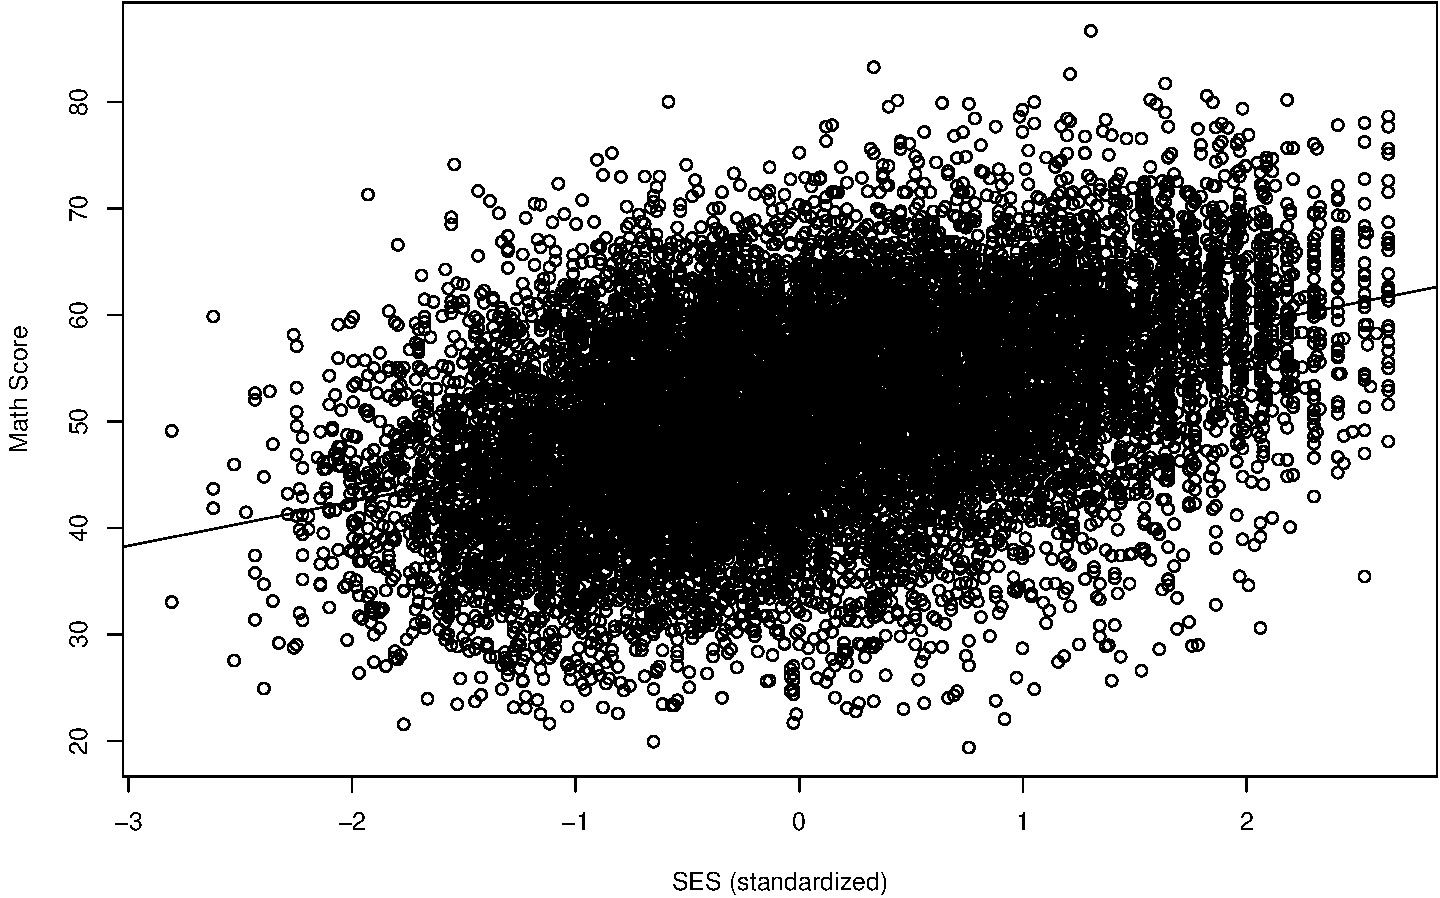
\includegraphics[width=0.8\linewidth]{anova_06_deck_files/figure-beamer/scatter-1}

\end{frame}

\begin{frame}{Big Picture}

Consider schools, which we represent using red, green, and blue points
on graphs, respectively. The schools we illustrate include one low SES
school, one middle SES school, and one high SES school.

Let's consider multiple ways in which we could obtain the marginal
association between SES and math score on the previous slide.

\end{frame}

\begin{frame}{}

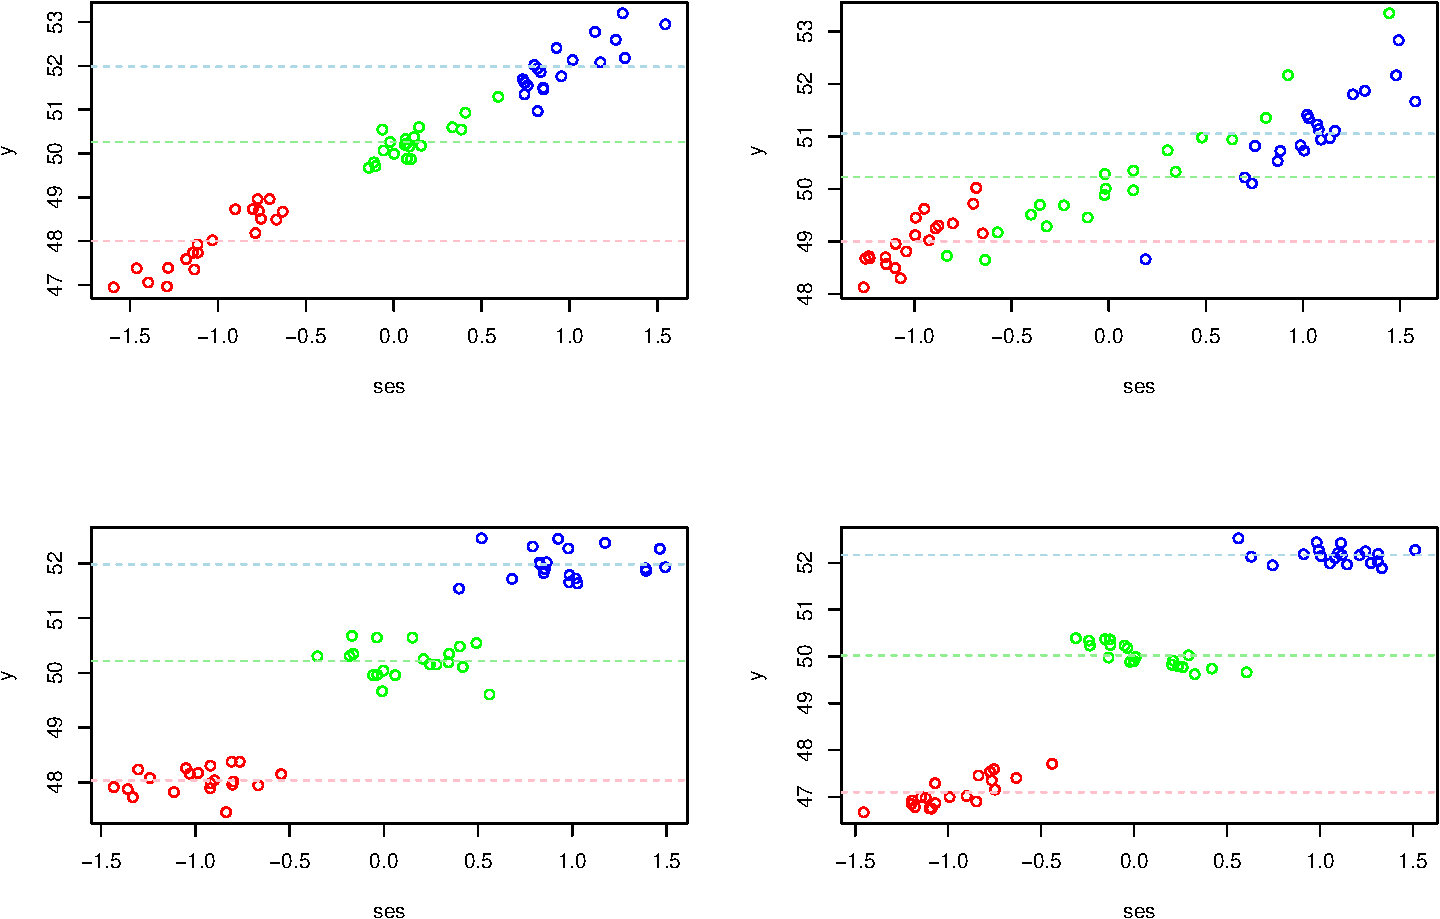
\includegraphics[width=0.6\linewidth]{anova_06_deck_files/figure-beamer/illustrateplot-1}

We want our model to be able to help us understand how SES (\(x_{ij}\))
and math scores are related in schools. In the framework of the model
\(y_{ij}=\beta_{0,j}+\beta_{1,j}x_{ij} + \varepsilon_{ij}\), what values
of \(\beta_{j}\) are consistent with these figures?

\end{frame}

\begin{frame}{}

One way to assess how SES is related to math score is to examine this
association in an ANCOVA model, allowing school-specific intercepts
while including SES as a covariate \(x_{ij}\):

\[y_{ij}=\beta_{0j}+\beta_1x_{ij} + \varepsilon_{ij}.\]

In this model, we estimate the same effect of SES for each school.

\end{frame}

\begin{frame}[fragile]{}

\begin{Shaded}
\begin{Highlighting}[]
\NormalTok{m5=}\KeywordTok{lmer}\NormalTok{(mscore}\OperatorTok{~}\NormalTok{sesstd}\OperatorTok{+}\NormalTok{(}\DecValTok{1}\OperatorTok{|}\NormalTok{school),}\DataTypeTok{data=}\NormalTok{nels_mathdat)}
\KeywordTok{summary}\NormalTok{(m5)}
\end{Highlighting}
\end{Shaded}

\begin{verbatim}
## Linear mixed model fit by REML ['lmerMod']
## Formula: mscore ~ sesstd + (1 | school)
##    Data: nels_mathdat
## 
## REML criterion at convergence: 92558.7
## 
## Scaled residuals: 
##     Min      1Q  Median      3Q     Max 
## -3.8753 -0.6428  0.0165  0.6693  4.4322 
## 
## Random effects:
##  Groups   Name        Variance Std.Dev.
##  school   (Intercept) 12.22    3.495   
##  Residual             68.03    8.248   
## Number of obs: 12974, groups:  school, 684
## 
## Fixed effects:
##             Estimate Std. Error t value
## (Intercept)  50.7175     0.1542  328.99
## sesstd        3.2900     0.0844   38.98
## 
## Correlation of Fixed Effects:
##        (Intr)
## sesstd -0.042
\end{verbatim}

This is a pretty big effect of SES -- a 1 SD increase in SES is
associated with a 2.7 point increase in math score on average.

\end{frame}

\begin{frame}[fragile]{}

\begin{Shaded}
\begin{Highlighting}[]
\KeywordTok{plot_model}\NormalTok{(m5,}\DataTypeTok{type=}\StringTok{'re'}\NormalTok{)}
\end{Highlighting}
\end{Shaded}

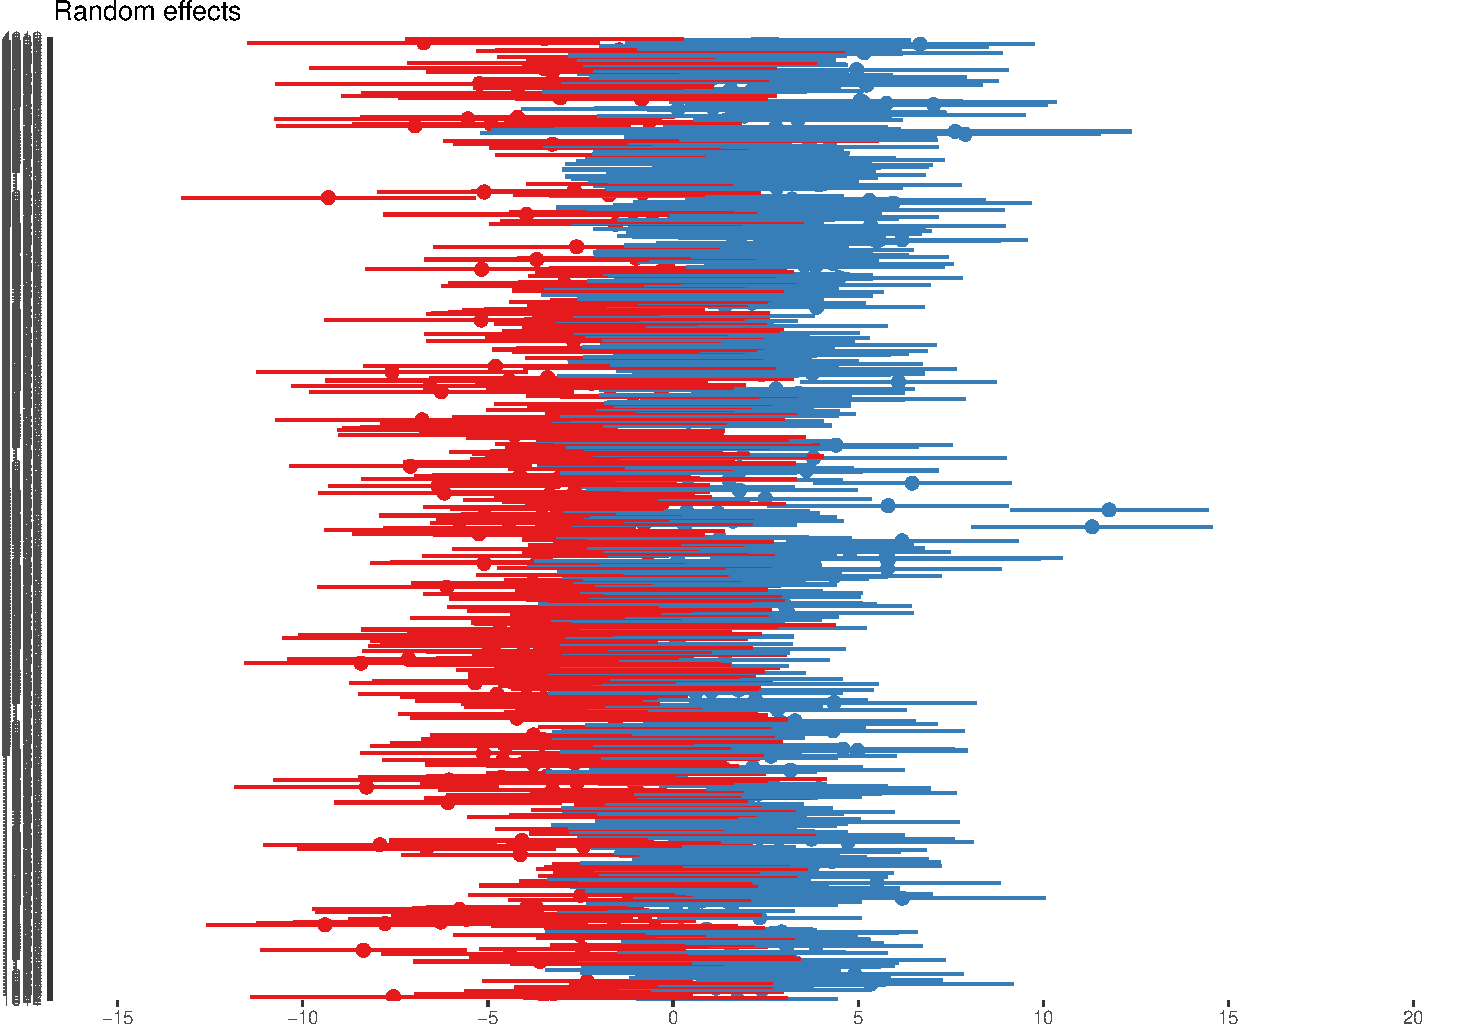
\includegraphics{anova_06_deck_files/figure-beamer/plotre3-1.pdf}

\end{frame}

\begin{frame}[fragile]{}

Let's plot the estimated school-specific lines from the random intercept
model.

\begin{Shaded}
\begin{Highlighting}[]
\NormalTok{xplot=}\KeywordTok{seq}\NormalTok{(}\OperatorTok{-}\FloatTok{2.9}\NormalTok{,}\FloatTok{2.3}\NormalTok{,}\DataTypeTok{by=}\NormalTok{.}\DecValTok{1}\NormalTok{)}
\NormalTok{yplot=}\KeywordTok{rep}\NormalTok{(}\DecValTok{60}\NormalTok{,}\KeywordTok{length}\NormalTok{(xplot))}
\KeywordTok{plot}\NormalTok{(xplot,yplot,}\DataTypeTok{type=}\StringTok{"n"}\NormalTok{,}\DataTypeTok{ylim=}\KeywordTok{c}\NormalTok{(}\DecValTok{30}\NormalTok{,}\DecValTok{70}\NormalTok{),}\DataTypeTok{xlab=}\StringTok{"Standardized SES"}\NormalTok{,}\DataTypeTok{ylab=}\StringTok{"Math Score"}\NormalTok{)}
\ControlFlowTok{for}\NormalTok{(school }\ControlFlowTok{in} \DecValTok{1}\OperatorTok{:}\KeywordTok{length}\NormalTok{(id.schools))}
\NormalTok{\{}
\NormalTok{  yplot=}\KeywordTok{coef}\NormalTok{(m5)}\OperatorTok{$}\NormalTok{school[school,}\DecValTok{1}\NormalTok{]}\OperatorTok{+}\KeywordTok{coef}\NormalTok{(m5)}\OperatorTok{$}\NormalTok{school[school,}\DecValTok{2}\NormalTok{]}\OperatorTok{*}\NormalTok{xplot}
  \KeywordTok{lines}\NormalTok{(xplot,yplot)}
\NormalTok{\}}
\end{Highlighting}
\end{Shaded}

\end{frame}

\begin{frame}{}

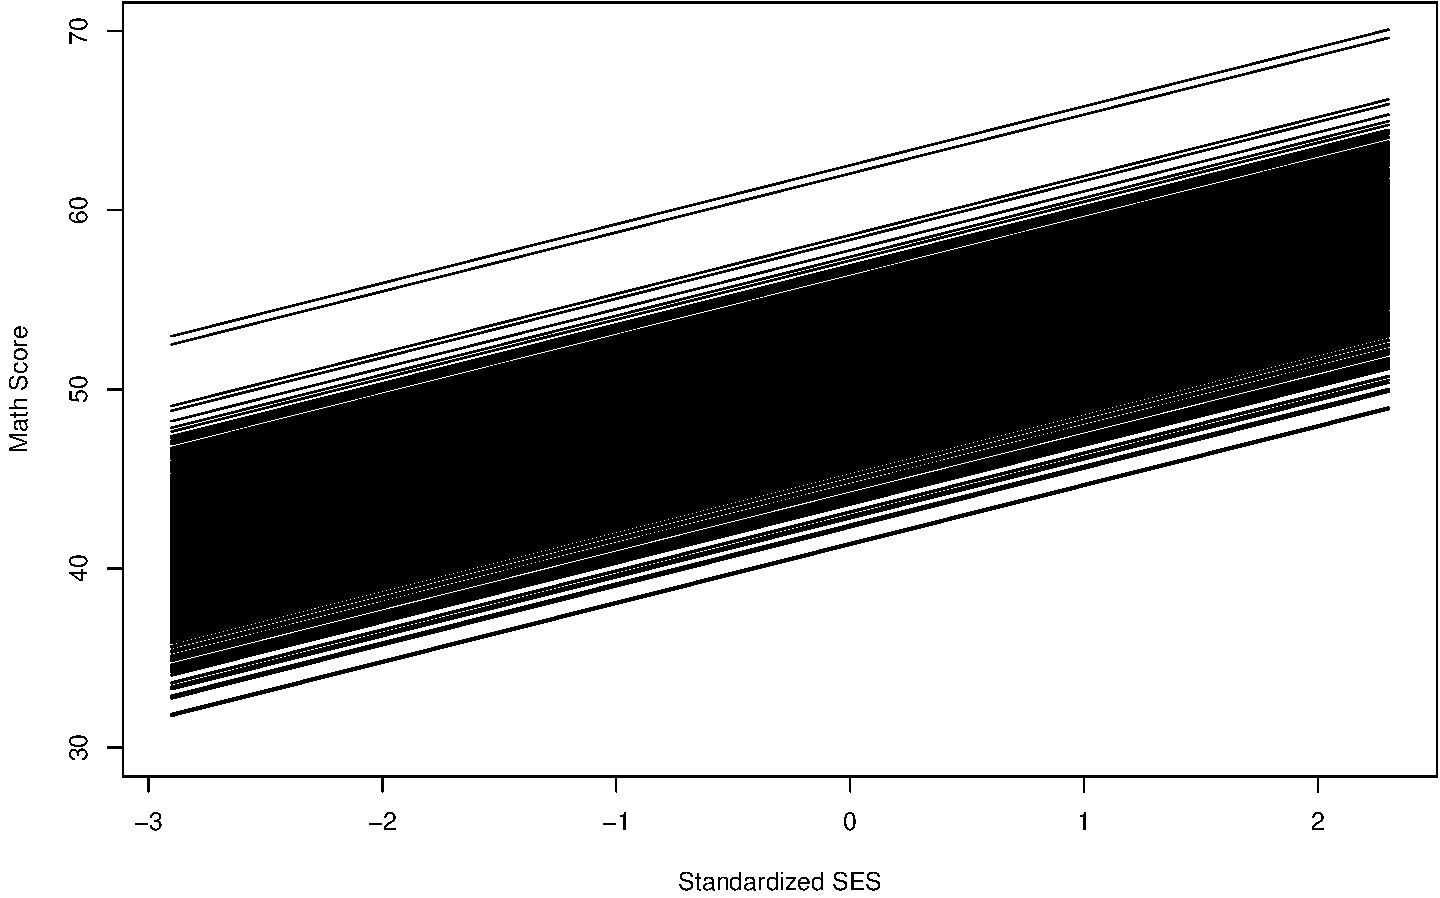
\includegraphics{anova_06_deck_files/figure-beamer/schoolspecific1b-1.pdf}

\end{frame}

\begin{frame}{}

This model allows separate intercepts for each school but assumes a
common slope. One concern is whether SES has the same relationship with
math scores in all schools. For example, some schools may have less of a
disparity in scores across levels of SES than others.

As an initial step, we can examine at variation in slopes across 100
separate regression models fit separately in each school:
\(y_{ij}=\beta_{0,j}+\beta_{1,j}x_{ij}+\varepsilon_{ij}, ~~ \varepsilon_{ij} \sim N(0,\sigma^2_j)\),
so that in each case \(\widehat{\beta}_j=(X_j'X_j)^{-1}X_j'y_j\), where
here \(X_j\) contains a column of 1's for the intercept and a column
containing the SES of each student.

\end{frame}

\begin{frame}{}

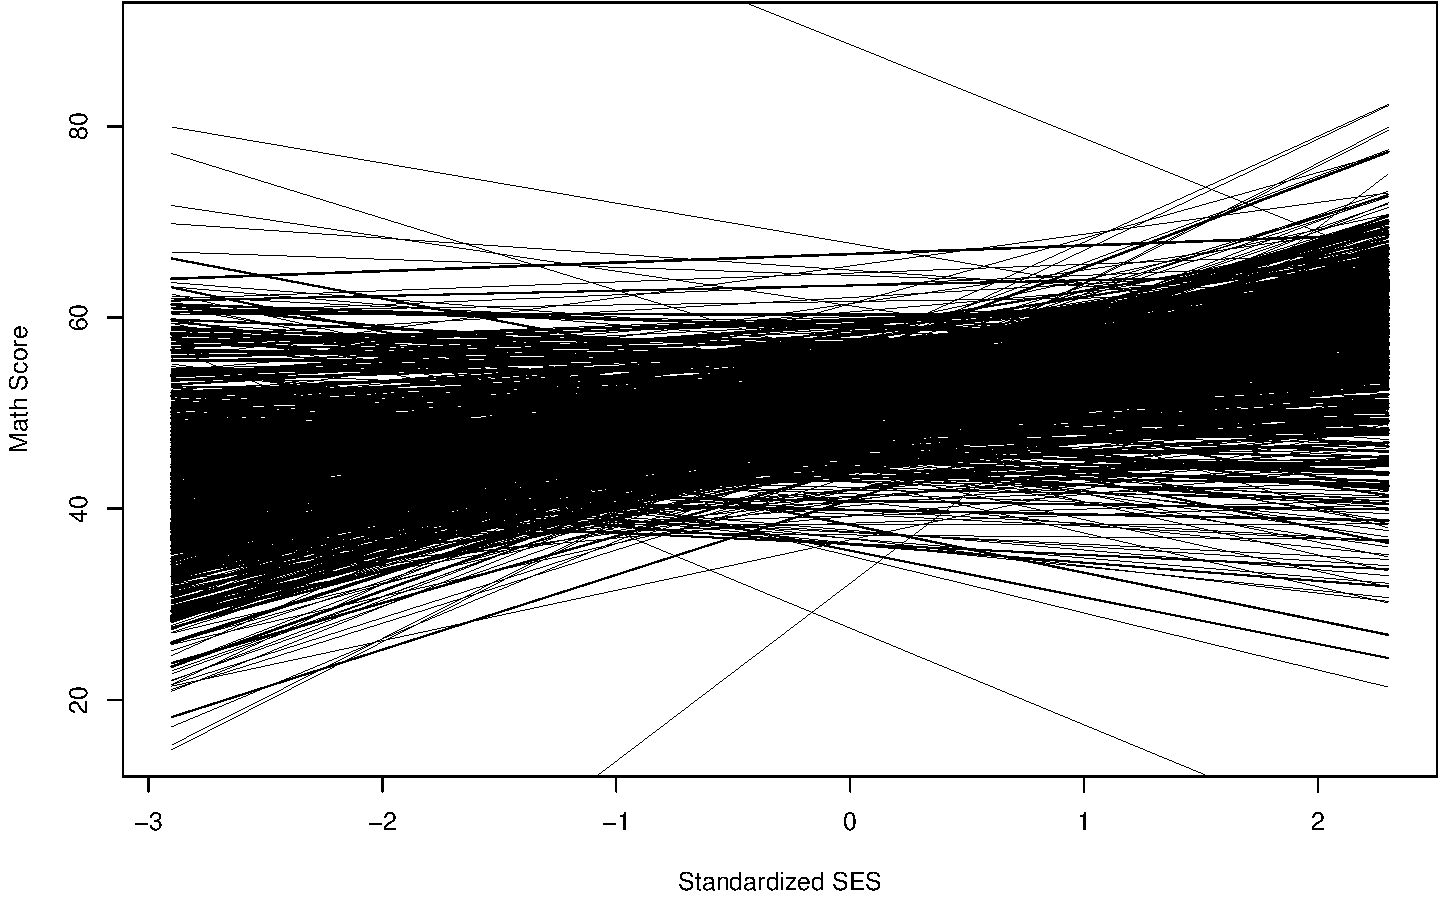
\includegraphics{anova_06_deck_files/figure-beamer/schoolspecific2b-1.pdf}

This plot looks pretty different!

\end{frame}

\begin{frame}{Histograms of school-specific intercepts and slopes}

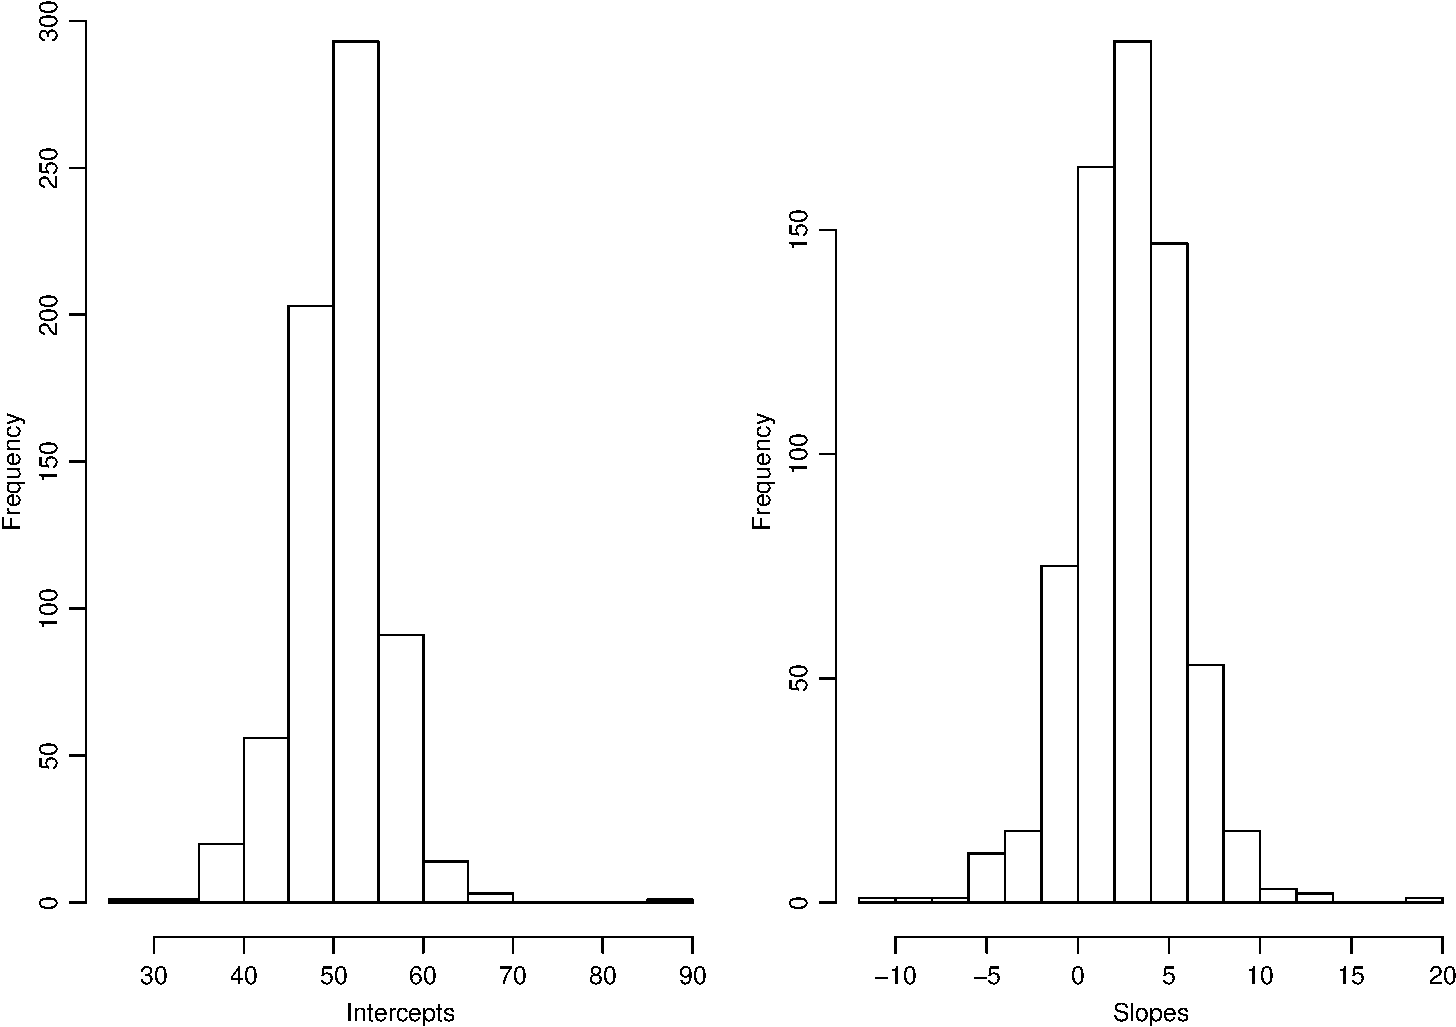
\includegraphics{anova_06_deck_files/figure-beamer/hist-1.pdf}

\end{frame}

\begin{frame}{}

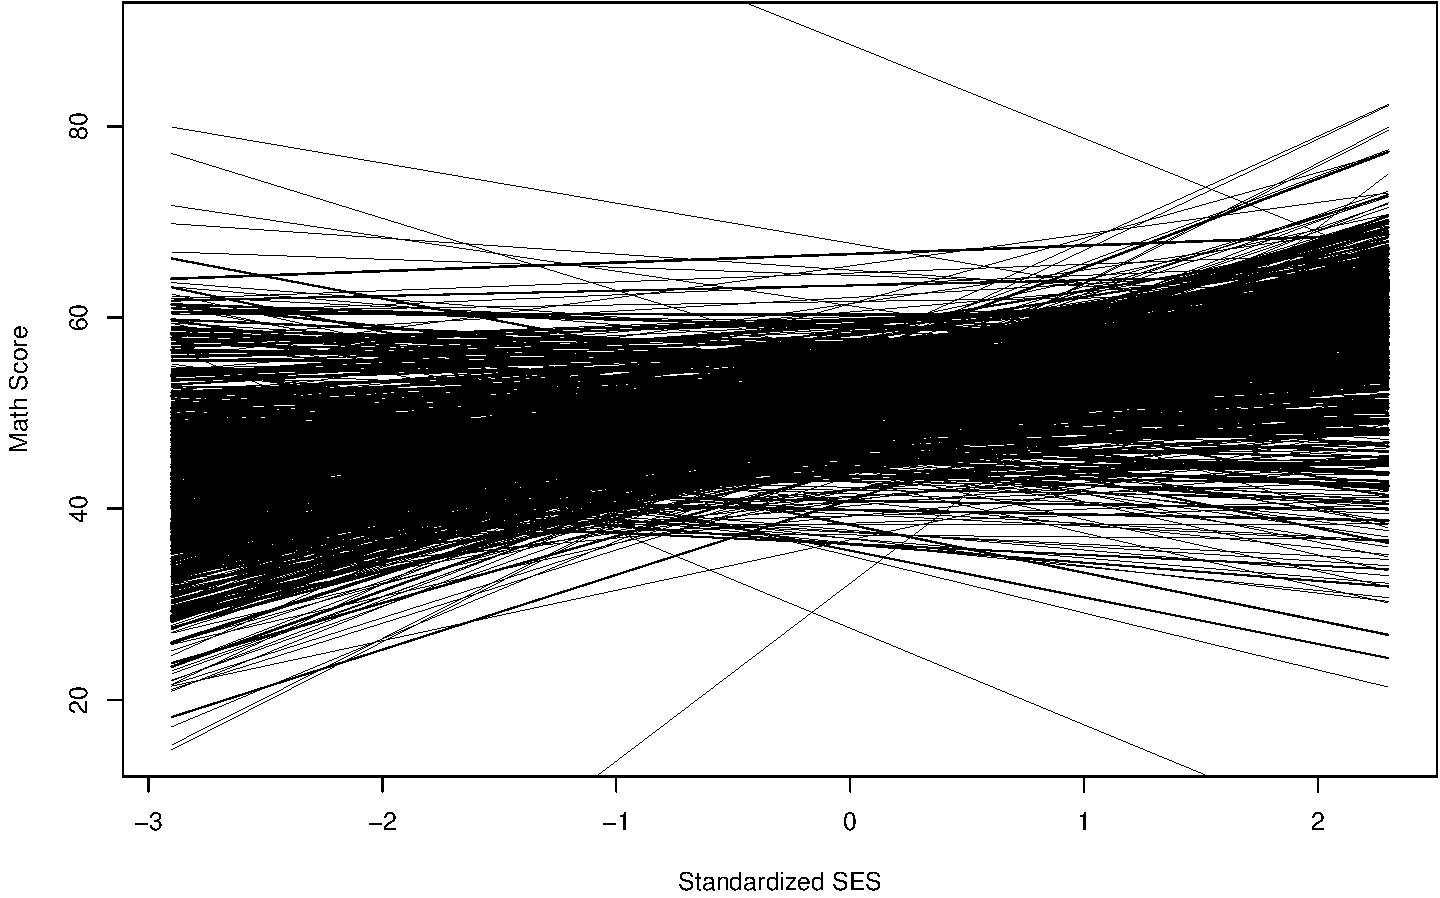
\includegraphics[width=0.5\linewidth]{anova_06_deck_files/figure-beamer/schoolspecific2c-1}

Line width is proportional to the number of students tested in each
school.

Of the 100 schools, 81 slopes are positive and 19 are negative. The
steepest slopes (positive and negative) tend to occur in the schools
with smaller sample sizes.

How do we get good estimates of the school-specific slopes?

\end{frame}

\begin{frame}{School-specific slopes}

Building on our knowledge of random intercept models, we could consider
the following estimates.

\begin{itemize}
\item
  \(\widehat{\beta}_j=\widehat{\beta}_j^{OLS}=(X_j'X_j)^{-1}X_j'y_j\),
  relying only on the data from school \(j\)
\item
  \(\widehat{\beta}_j=\widehat{\beta}^{POOL}=(X'X)^{-1}X'y\), using all
  the data and pooling across schools
\item
  \(\widehat{\beta}_j=w_j\widehat{\beta}_j^{OLS} + (1-w_j)\widehat{\beta}^{POOL}\),
  doing something in between
\end{itemize}

\end{frame}

\begin{frame}{School-specific slopes}

One alternative to separate linear regression models for each school is
fitting a single model with school-specific slopes and intercepts. These
factors could be fixed or random effects. First, let's consider the
fixed effects approach.

\[y_{ij}=\beta_{0,j}+\beta_{1,j}x_{ij}+\varepsilon_{ij}, ~~~ \varepsilon_{ij} \sim N(0,\sigma^2)\]

If we wish to evaluate whether there is heterogeneity across schools, an
easy approach is to fit the model as a linear regression using indicator
variables as follows.

\end{frame}

\begin{frame}{}

\[y_{ij}=\beta_0+\alpha_jI(\text{school}=j) + \beta_1x_{ij} + \gamma_jx_{ij}I(\text{school}=j) + \varepsilon_{ij},\]
where we assume \(\alpha_J=\gamma_J=0\) (reference cell coding).

In this case, a (J-1) df test can be used to evaluate the hypothesis

\[H_0: \gamma_j=0,~~~ j=1,\ldots,J-1,\]

which corresponds to a constant effect of SES, \(\beta_1\), across
groups.

\end{frame}

\begin{frame}[fragile]{}

\begin{Shaded}
\begin{Highlighting}[]
\NormalTok{m6=}\KeywordTok{lm}\NormalTok{(nels_mathdat}\OperatorTok{$}\NormalTok{mscore}\OperatorTok{~}\KeywordTok{as.factor}\NormalTok{(nels_mathdat}\OperatorTok{$}\NormalTok{school)}\OperatorTok{+}\NormalTok{nels_mathdat}\OperatorTok{$}\NormalTok{sesstd) }\CommentTok{#pooled slope}
\NormalTok{m7=}\KeywordTok{lm}\NormalTok{(nels_mathdat}\OperatorTok{$}\NormalTok{mscore}\OperatorTok{~}\KeywordTok{as.factor}\NormalTok{(nels_mathdat}\OperatorTok{$}\NormalTok{school)}\OperatorTok{+}\NormalTok{nels_mathdat}\OperatorTok{$}\NormalTok{sesstd}\OperatorTok{+}\KeywordTok{as.factor}\NormalTok{(nels_mathdat}\OperatorTok{$}\NormalTok{school)}\OperatorTok{*}\NormalTok{nels_mathdat}\OperatorTok{$}\NormalTok{sesstd) }\CommentTok{#school-specific slopes}
\NormalTok{LR=}\DecValTok{2}\OperatorTok{*}\NormalTok{(}\KeywordTok{logLik}\NormalTok{(m7)}\OperatorTok{-}\KeywordTok{logLik}\NormalTok{(m6))}
\DecValTok{1}\OperatorTok{-}\KeywordTok{pchisq}\NormalTok{(LR,}\DecValTok{201}\OperatorTok{-}\DecValTok{102}\NormalTok{)}
\end{Highlighting}
\end{Shaded}

\begin{verbatim}
## 'log Lik.' 0 (df=1368)
\end{verbatim}

Here we have evidence in favor of school-specific slopes in the fixed
effects model. However, our estimates of school-specific slopes in small
schools may have high variance.

\end{frame}

\begin{frame}{}

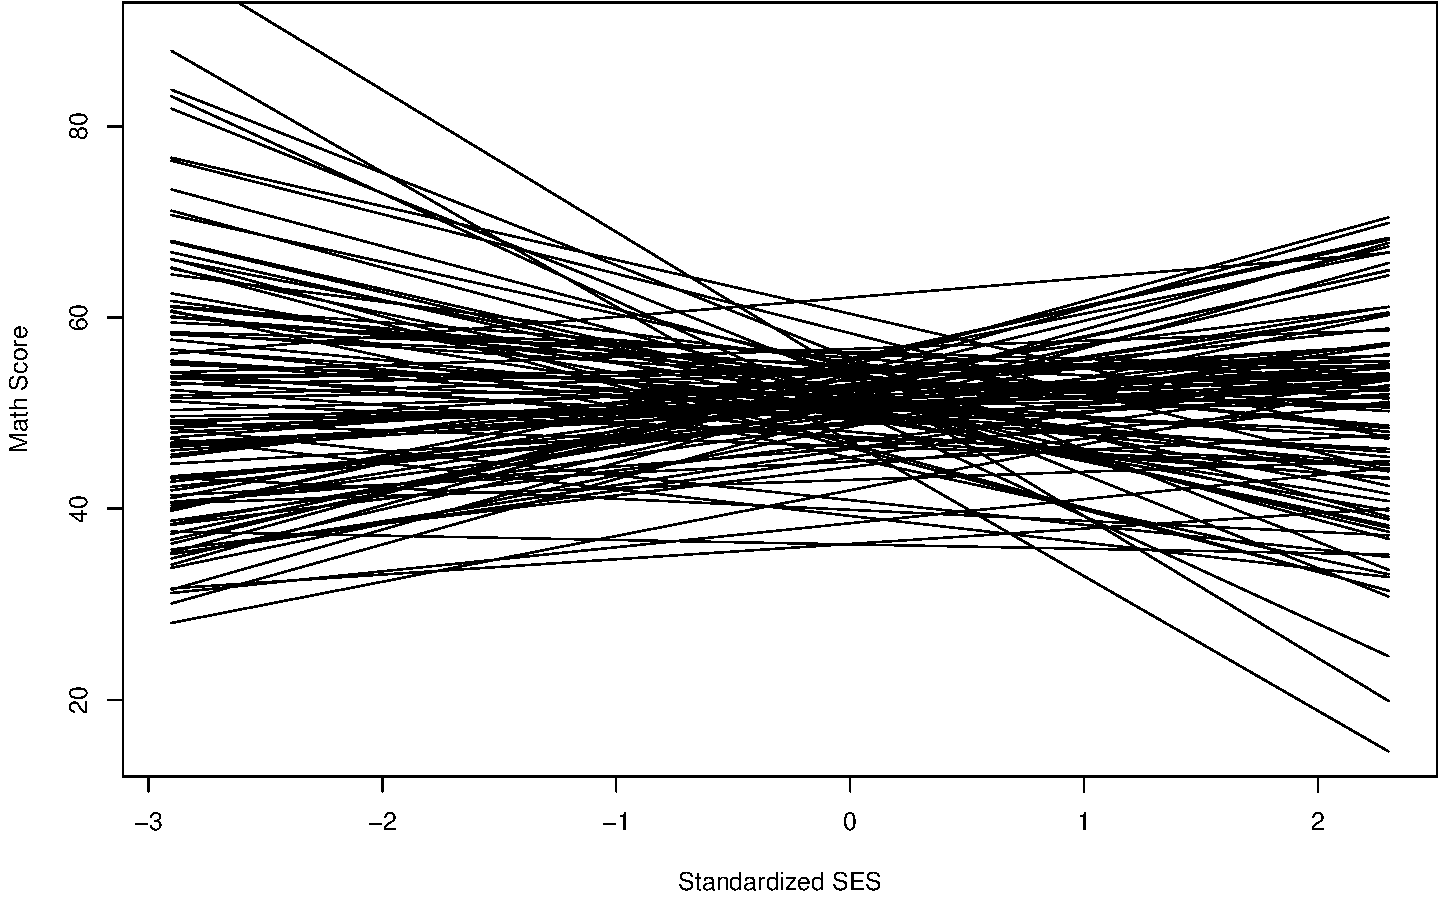
\includegraphics{anova_06_deck_files/figure-beamer/plotslopes-1.pdf}

The only difference from the models used to obtain the prior lines is
that in this case we estimated a common variance.

\end{frame}

\begin{frame}{}

How should we estimate \(\beta_j\)? Is this pattern becoming familiar?

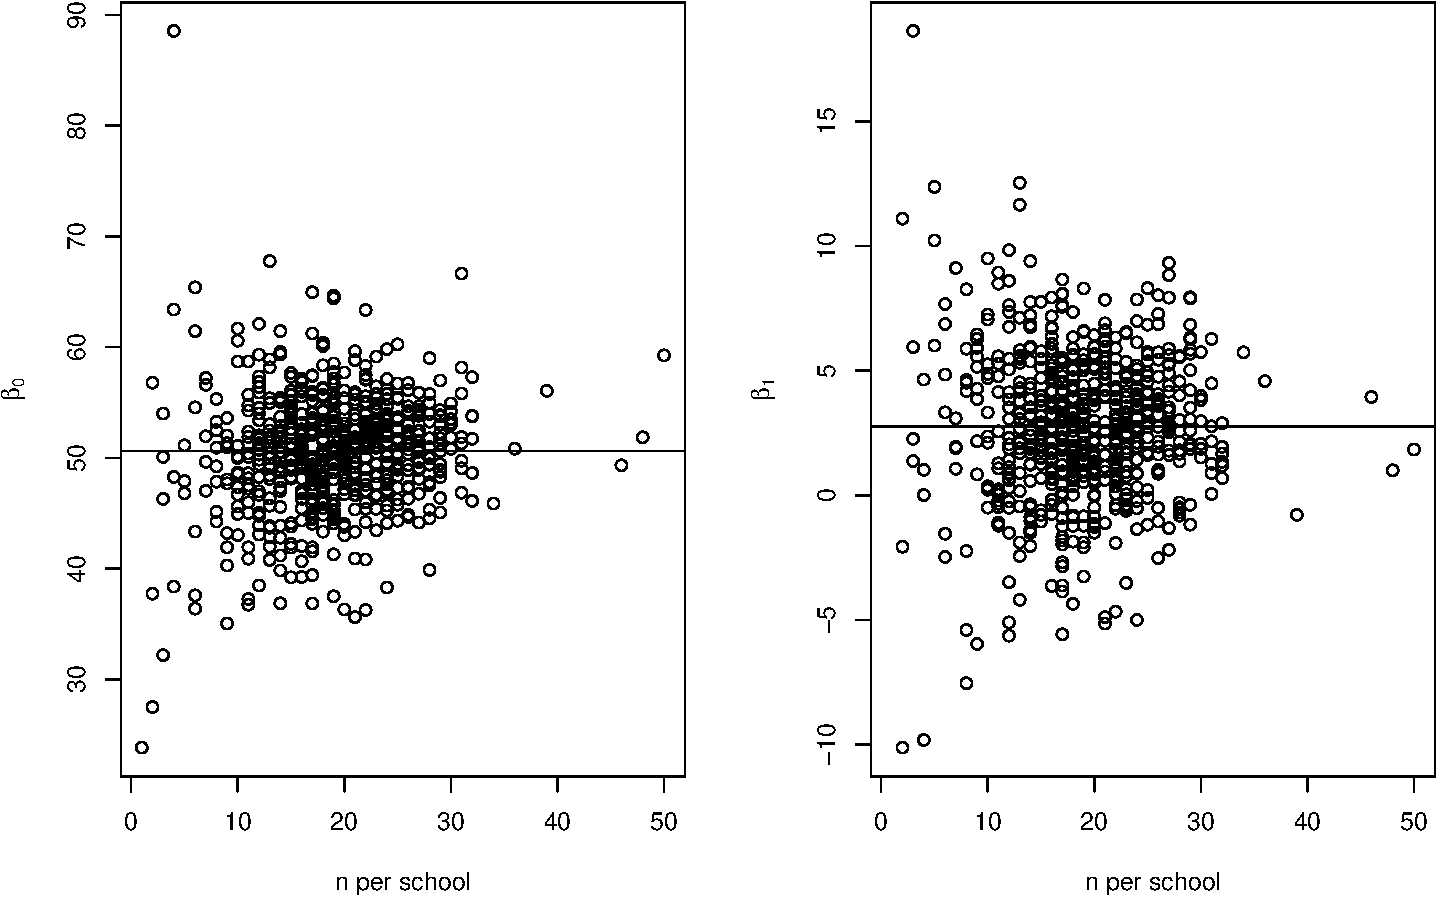
\includegraphics{anova_06_deck_files/figure-beamer/betasbyn-1.pdf}

\end{frame}

\begin{frame}{Hierarchical Regression Models}

Our hierarchical normal model involves two levels:

\begin{itemize}
\tightlist
\item
  within-group model \(p(y_{1j},\ldots,y_{n_jj} \mid \theta_j)\)
  describing heterogeneity in group j
\item
  among-groups model \(p(\theta_1,\ldots,\theta_J)\)
\end{itemize}

Specifically, we let

\begin{itemize}
\tightlist
\item
  \(\theta_j=(\mu_j, \sigma^2)\)
\item
  \(y_{1j}, \ldots y_{n_jj} \mid \theta \overset{iid}{\sim}N\left(\mu_j, \sigma^2\right)\)
\item
  \(\mu_1,\ldots,\mu_j \overset{iid}{\sim}N\left(\mu, \tau^2\right)\)
\end{itemize}

\end{frame}

\begin{frame}{}

In the regression setting, we have

\begin{itemize}
\tightlist
\item
  \(\theta_j=(\beta_j, \sigma^2)\)
\item
  \(y_{ij}=\beta_j'x_{ij}+\varepsilon_{ij}, ~~ \varepsilon_{ij} \overset{iid}{\sim} N\left(0,\sigma^2\right)\)
\item
  \(\beta_1, \ldots, \beta_J \overset{iid}{\sim} p(\beta_j)\)
\end{itemize}

How should we model \(p(\beta_j)\), the heterogeneity across groups in
the vector of regression coefficients?

\end{frame}

\begin{frame}{}

It is often the case that intercepts and slopes are correlated.

\begin{itemize}
\tightlist
\item
  In a study of income over time, people who start off making more money
  may have larger raises over time.
\item
  In a study of exercise, people who exercise a lot at the start of the
  study may have lower changes over time than those who exercise less
\end{itemize}

A natural choice for the \(\beta_j\) model is the multivariate normal
distribution, which allows for correlation among the group-specific
regression coefficients.

\end{frame}

\begin{frame}{}

We can specify our model in the context of maximum likelihood estimation
as

\begin{itemize}
\tightlist
\item
  \(y_j \mid \beta_j \sim MVN(X_j\beta_j, \sigma^2I)\)
\item
  \(\beta_j \sim MVN(\beta,\Sigma_\beta)\)
\end{itemize}

\(\beta_j \sim MVN(\beta,\Sigma_\beta) \iff \beta_j=\beta+b_j, ~~ b_j \sim MVN(0, \Sigma_\beta)\)

The parameters are

\begin{itemize}
\tightlist
\item
  \(\beta\), an across-group mean vector of regression coefficients
\item
  \(\Sigma_\beta\), a covariance matrix describing the variability of
  the \(\beta_j\) around \(\beta\)
\end{itemize}

\end{frame}

\begin{frame}{}

We can combine terms and write the model as

\[y_j=X_j\beta_j+\varepsilon_j=X_j(\beta+b_j)+\varepsilon_j=X_j\beta+x_jb_j+\varepsilon_j\]

Here

\begin{itemize}
\tightlist
\item
  \(\beta\) is sometimes called a fixed effect (fixed across all groups)
\item
  \(b_j\) is sometimes called a random effect (varies across groups and
  can be considered random if groups were randomly sampled)
\item
  a model with both fixed and random effects is often called a
  mixed-effects model
\end{itemize}

\end{frame}

\begin{frame}[fragile]{\emph{Ad hoc} estimates}

We can get a rough estimate of \(\beta\) by averaging the estimates from
our 100 school-specific regression models.

\begin{Shaded}
\begin{Highlighting}[]
\KeywordTok{apply}\NormalTok{(BETA.OLS,}\DecValTok{2}\NormalTok{,mean)}
\end{Highlighting}
\end{Shaded}

\begin{verbatim}
## (Intercept)          xj 
##    50.61823          NA
\end{verbatim}

This estimator is not perfect -- it equally weights all the schools,
regardless of size. We would prefer to assign a lower weight to schools
with less data.

\end{frame}

\begin{frame}[fragile]{\emph{Ad hoc} estimates}

We can get a \emph{very rough} estimate of \(\Sigma_\beta\):

\begin{Shaded}
\begin{Highlighting}[]
\KeywordTok{cov}\NormalTok{(BETA.OLS,}\DataTypeTok{use=}\StringTok{"complete.obs"}\NormalTok{) }\CommentTok{#dropped n=1 schools}
\end{Highlighting}
\end{Shaded}

\begin{verbatim}
##             (Intercept)        xj
## (Intercept)  26.7958507 0.7529181
## xj            0.7529181 8.9391754
\end{verbatim}

This estimate not only ignores sample size differences, it also ignores
the variability of \(\widehat{\beta}_j\) around \(\beta_j\):
\[\text{Var}[\widehat{\beta}_j\text{'s around }\widehat{\beta}] \approx \text{Var}[\beta_j\text{'s around }\beta]+\text{Var}[\widehat{\beta}_j\text{'s around }\beta_j\text{'s}]:\]

basically, the sample covariance of the \(\widehat{\beta}_j\)'s is
approximately \[\Sigma_\beta +  \text{estimation error}\]

\end{frame}

\begin{frame}{Covariance within Groups}

\(Cov(y_j)=E[(y_j-E(y_j))(y_j-E(y_j))']\)

In our model
\[y_j=X_j\beta_j+\varepsilon_j=X_j(\beta+b_j)+\varepsilon_j=X_j\beta+x_jb_j+\varepsilon_j\],
\[y_j-E[y_j]=y_j-X_j\beta=X_jb_j+\varepsilon_j,~~ $b_j \sim N(0,\Sigma_\beta), ~~\varepsilon_j \sim N(0,\sigma^2I)\]
and because we specify \(b_j \perp \varepsilon_j\),
\[Cov(y_j)=E[(X_jb_j+\varepsilon_j)(X_jb_j+\varepsilon_j)']\]
\[=E[X_jb_jb_j'X_j']+E[\varepsilon_j\varepsilon_j']=X_j\Sigma_\beta X_j'+\sigma^2I.\]

\end{frame}

\begin{frame}{Marginal and conditional distributions of \(y\)}

So conditional on \(b_j\), \[y_j \sim MVN(X_j\beta+X_jb_j, \sigma^2I)\]
and unconditional on \(b_j\) we have
\[p(y_j \mid \beta, \Sigma_\beta, \sigma^2)=MVN(X_j\beta, X_j\Sigma_\beta X_j' + \sigma^2I).\]

\end{frame}

\begin{frame}{Dependence and conditional independence}

Marginal dependence: If we don't know \(\beta_j\) (or \(b_j\)), then
knowing the response \(y_{ij}\) gives me some information about
\(\beta_j\), which gives us some information about \(y_{i'j}\), so the
observations within a group are dependent.

Conditional independence: If I do know \(\beta_j\), then knowing
\(y_{ij}\) does not give me any extra information about \(y_{i'j}\), and
they are independent. My information about \(y_{ij} \perp y_{i'j}\) if I
know \(\beta_j\).

\end{frame}

\begin{frame}[fragile]{Fitting the model}

\begin{Shaded}
\begin{Highlighting}[]
\CommentTok{#recall g.nels is the sequential ID variable}
\NormalTok{m8=}\KeywordTok{lmer}\NormalTok{(nels_mathdat}\OperatorTok{$}\NormalTok{mscore}\OperatorTok{~}\NormalTok{nels_mathdat}\OperatorTok{$}\NormalTok{sesstd}\OperatorTok{+}\NormalTok{(nels_mathdat}\OperatorTok{$}\NormalTok{sesstd}\OperatorTok{|}\NormalTok{g.nels),}\DataTypeTok{REML=}\OtherTok{FALSE}\NormalTok{)}
\KeywordTok{summary}\NormalTok{(m8)}
\end{Highlighting}
\end{Shaded}

\begin{verbatim}
## Linear mixed model fit by maximum likelihood  ['lmerMod']
## Formula: 
## nels_mathdat$mscore ~ nels_mathdat$sesstd + (nels_mathdat$sesstd |  
##     g.nels)
## 
##      AIC      BIC   logLik deviance df.resid 
##  92553.1  92597.9 -46270.5  92541.1    12968 
## 
## Scaled residuals: 
##     Min      1Q  Median      3Q     Max 
## -3.8910 -0.6382  0.0179  0.6669  4.4613 
## 
## Random effects:
##  Groups   Name                Variance Std.Dev. Corr
##  g.nels   (Intercept)         12.2231  3.4961       
##           nels_mathdat$sesstd  0.8562  0.9253   0.11
##  Residual                     67.3451  8.2064       
## Number of obs: 12974, groups:  g.nels, 684
## 
## Fixed effects:
##                     Estimate Std. Error t value
## (Intercept)         50.67670    0.15511   326.7
## nels_mathdat$sesstd  3.27708    0.09256    35.4
## 
## Correlation of Fixed Effects:
##             (Intr)
## nls_mthdt$s 0.007
\end{verbatim}

\end{frame}

\begin{frame}[fragile]{Do we need the random slope in addition to the
random intercept?}

Let's test whether the slope should be random or fixed -- this time the
reference distribution is a 50-50 mixture of \(\chi^2_1\) and
\(\chi^2_2\) distributions. This is a test of the hypothesis that the
variance of the random slope is zero.

\begin{Shaded}
\begin{Highlighting}[]
\NormalTok{LR=}\KeywordTok{logLik}\NormalTok{(}\KeywordTok{lmer}\NormalTok{(mscore}\OperatorTok{~}\NormalTok{(}\DecValTok{1}\OperatorTok{|}\NormalTok{school),}\DataTypeTok{data=}\NormalTok{nels_mathdat,}\DataTypeTok{REML=}\OtherTok{FALSE}\NormalTok{))}
 \OperatorTok{-}\KeywordTok{logLik}\NormalTok{(}\KeywordTok{lmer}\NormalTok{(mscore}\OperatorTok{~}\NormalTok{sesstd}\OperatorTok{+}\NormalTok{(sesstd}\OperatorTok{|}\NormalTok{school),}
              \DataTypeTok{data=}\NormalTok{nels_mathdat,}\DataTypeTok{REML=}\OtherTok{FALSE}\NormalTok{))}
\end{Highlighting}
\end{Shaded}

\begin{verbatim}
## 'log Lik.' 46270.53 (df=6)
\end{verbatim}

\begin{Shaded}
\begin{Highlighting}[]
\FloatTok{0.5}\OperatorTok{*}\NormalTok{(}\DecValTok{1}\OperatorTok{-}\KeywordTok{pchisq}\NormalTok{(LR[}\DecValTok{1}\NormalTok{],}\DecValTok{2}\NormalTok{)}\OperatorTok{+}\DecValTok{1}\OperatorTok{-}\KeywordTok{pchisq}\NormalTok{(LR[}\DecValTok{1}\NormalTok{],}\DecValTok{1}\NormalTok{))}
\end{Highlighting}
\end{Shaded}

\begin{verbatim}
## [1] 1
\end{verbatim}

Yes, looks like the random slope explains additional variance.

\end{frame}

\end{document}
